%% Submissions for peer-review must enable line-numbering 
%% using the lineno option in the \documentclass command.
%%
%% Preprints and camera-ready submissions do not need 
%% line numbers, and should have this option removed.
%%
%% Please note that the line numbering option requires
%% version 1.1 or newer of the wlpeerj.cls file, and
%% the corresponding author info requires v1.2

\documentclass[fleqn,10pt,lineno]{wlpeerj} % for journal submissions
%\documentclass[fleqn,10pt]{wlpeerj} % for preprint submissions
%%%%%%%%%%%%%%%%%%%%%%%%%%%%%%%%%%%%%%%%%%%%%%%%%%%%%%%%%%%%%%%%%%%%%%%%%%%%%%%%
% USER DEFINED PACKAGES
%%%%%%%%%%%%%%%%%%%%%%%%%%%%%%%%%%%%%%%%%%%%%%%%%%%%%%%%%%%%%%%%%%%%%%%%%%%%%%%%
\usepackage[utf8]{inputenc}
\usepackage[T1]{fontenc}
\usepackage[english]{babel}
\usepackage{textcomp}% for '\textdegree' macro
\usepackage{graphicx}
\usepackage{float}
%\usepackage[tight,footnotesize]{subfigure}
\usepackage{subcaption}
\usepackage{tabularx}
\usepackage{makecell}
\usepackage{multirow}
\graphicspath{{images/}}








%%%%%%%%%%%%%%%%%%%%%%%%%%%%%%%%%%%%%%%%%%%%%%%%%%%%%%%%%%%%%%%%%%%%%%%%%%%%%%%%
\title{A semi-automatic tool to geolocalize historical landscape images}

% \keywords{Keyword1, Keyword2, Keyword3}



\begin{abstract}
Smapshot is a web-based participatory virtual globe \citep{produit2018} where  
users can georeference historical images of the landscape by clicking a minimum
of six well identifiable correspondence points between the image and a 3D virtual 
globe.
% The image is then superimposed with the 3D model giving the impression that
% the observer is looking through a window of the past. 
The images database is expected to grow exponentially. In a near future, 
the work of the web users will no longer be enough.

To tackle this issue, we developed a semi-automatic process to georeference images.
The volunteers will be shown only images having a maximum number of neighbour images 
in the matching graph. These neighbour images are the ones with which they share 
some overlay. 
This overlap is detected using the SIFT algorithm \citep{lowe1999} in a pairewise 
matching process.

For an image pair made of a reference image with a known pose and a query image 
we want to georeference, we extracted the 3D world coordinates of the tie points
from a digital elevation model.

Then, by running a perspective-n-point algorithm after having geometrically tested the
resulting homography between the two images, we compute the 6 degree of freedom pose,
i.e. the position (X,Y,Z) and orientation (azimuth, tilt and roll angles) of the 
query image. The query image then becomes a reference and the georeference 
computation can be propagated more deeply in the graph structure.
\end{abstract}



%%%%%%%%%%%%%%%%%%%%%%%%%%%%%%%%%%%%%%%%%%%%%%%%%%%%%%%%%%%%%%%%%%%%%%%%%%%%%%%%
%%%%%%%%%%%%%%%%%%%%%%%%%%%%%%%%%%%%%%%%%%%%%%%%%%%%%%%%%%%%%%%%%%%%%%%%%%%%%%%%
\begin{document}

\flushbottom
\maketitle
\thispagestyle{empty}

%%%%%%%%%%%%%%%%%%%%%%%%%%%%%%%%%%%%%%%%%%%%%%%%%%%%%%%%%%%%%%%%%%%%%%%%%%%%%%%%
\section*{Introduction}
%%%%%%%%%%%%%%%%%%%%%%%%%%%%%%%%%%%%%%%%%%%%%%%%%%%%%%%%%%%%%%%%%%%%%%%%%%%%%%%%
Smapshot is a web-based participatory virtual globe. It uses crowdsourcing for 
the georeferencing of historical images. These images come from various sources, 
such as public archives or private libraries. Volunteers georeference images 
they know a prior coarse location by picking a minimum of six identifiable 
correspondence points both in the image and the textured 3D model of the landscape. 
A pose estimation algorithm computes the position and orientation of the camera 
and the image is then superimposed  with the 3D model giving the impression that 
the observer is looking through a window of the past.

As every other online image databases, the smapshot one is expected to 
exponentially grow in a near future. The georeferencing of the images currently 
carried out by volunteer Internet users will no longer be enough.
In order to considerably simplify their task, this work introduces a method to
geolocate images in a semi-automatic way.

%%%%%%%%%%%%%%%%
\iffalse
This study shows that it is possible 
to classify images by different methods. Content based image retrieval % (CBIR) 
makes use of merging local and global features of an image as a multidimensional 
vector \citep{smeulders2000}. 
This vector is then compared (much more faster than the image itself) with 
a database to search for the similar other vectors and thus, images. 
Object retrieval can also be used for spatial matching between images 
\citep{philbin2007}.

Bag-of-Features is another technique that reduces the space of the many 
features of an image to a simple histogram \citep{feifei2005}. 
It is then easier to find or compare images solely based on it. 
Supervised learning techniques can then be used to classify images.
However, they require a training phase that is time consuming and need 
significant computational resources.

But there is one more step to achieve to geolocate images. 
\fi
%%%%%%%%%%%%%%%%


Some studies have shown it is possible to geolocate large quantities of 
images only based on their comparison with a database of millions of geotagged 
images \citep{hays2015,weyand2016}. Object retrieval technique can also be used 
for spatial matching between images \citep{philbin2007}. 
\cite{baatz2012} have used a sky segmentation method in mountaineous terrain 
to extract contour informations and matched them with DEM data using a 
bag-of-word approach \citep{feifei2005}. \cite{produit2014} also makes use
of a Kalman filter robust skyline matching approach with an initial user input 
to compute the pose of an image.


In recent years, deep learning methods such as convolutional neural networks 
\citep{lecun2015deep} have shown that they are also very well suited to classifying 
or searching images in very large databases, even for geolocation purposes \citep{weyand2016}.

This work brings an optimization method in volunteers based image georeferencing.
They will only be shown central images in a pairewise matching graph. 
The geolocation they provide to these central images will then be automatically 
propagated to other images in the graph in a 4 stages iteration process involving:
1) a pairewise image matching to find images with overlay, 
2) the extraction of highest valency images (i.e. central images) on the 
pairewise resulting graph, 
3) the georeferencing of central images by volunteers, 
4) the automatic georeferencing of images sharing overlay with the user 
georeferenced central ones.
%%%%%%%%%%%%%%%%
\iffalse
\begin{enumerate}\itemsep0.2em
\item a pairewise image matching to find images with overlay
\item the extraction of highest valency images (i.e. central images) on the 
pairewise resulting graph
\item the georeferencing of central images by volunteers
\item the automatic georeferencing of images sharing overlay with the user 
georeferenced central ones
\end{enumerate}
\fi
%%%%%%%%%%%%%%%%
%It also proposes a way to insert this approach in a user friendly way on the 
%existing plateform.


%%%%%%%%%%%%%%%%%%%%%%%%%%%%%%%%%%%%%%%%%%%%%%%%%%%%%%%%%%%%%%%%%%%%%%%%%%%%%%%%
\section*{Method}
%%%%%%%%%%%%%%%%%%%%%%%%%%%%%%%%%%%%%%%%%%%%%%%%%%%%%%%%%%%%%%%%%%%%%%%%%%%%%%%%
%To evaluate the method, we first build a sample dataset.
%%%%%%%%%%%%%%%%%%%%%%%%%%%%%%%%%%%%%%%%
\subsection*{Building a sample dataset}
%%%%%%%%%%%%%%%%%%%%%%%%%%%%%%%%%%%%%%%%
All images come from the smapshot database and are already geolocated. 
This geolocation was manually verified prior to the work. 
Therefore their position and orientation can be used; 
1) as a ground truth to  validate and evaluate the geolocation computation and 
2) to build sets of images having high chances to show some overlay, 
which is intended to drastically reduce the calculation time. 
To build such subsets we have run  the DBSCAN clustering algorithm 
\citep{ester1996} on the database.

%%%%%%%%%%%%%%%%%%%%%%%%%%%%%%%%%%%%%%%%
\subsection*{Computation steps}
%%%%%%%%%%%%%%%%%%%%%%%%%%%%%%%%%%%%%%%%


\subsubsection*{Local features extraction and images matching}
%%%%%%%%%%%%%%%%%%%%%%%%%%%%%%%%%%%%%%%%
In a first stage, 
the method used consists by first computing local images descriptors on all 
images of a sample. 
Then, we used SIFT and its pairewise image matching algorithm based on the 
similarities of their descriptor \citep{lowe1999}. 
Since descriptors are fixed dimension vectors, these similarities also characterize 
the distances between them within the descriptors space. 
By applying RANSAC \citep{fischler1981} to compute the homography matrix for each 
image pair, we are able remove some false positive in this first matching results.
 

\subsubsection*{Geometrical filter}
%%%%%%%%%%%%%%%%%%%%%%%%%%%%%%%%%%%%%%%%
Finally, in order to eliminate the last false positive results, we developed 
a geometrical filter.
This filter works as follow: we first compute the projection of the frame of the first
image onto the second one using the  homography matrix computed with RANSAC and then
we make some simple tests on this geometry. These tests only retains geometries with:
1) a non-intersecting shape
2) a convexe shape
3) a shape surface representing at least 10\% of the image.
%%%%%%%%%%%%%%%%
\iffalse
\item a non-intersecting shape
\item a convexe shape
\item a shape surface representing at least 10\% of the image.
\fi
%%%%%%%%%%%%%%%%
%Finally, in order to eliminate the last outliers, we developed a filter based
%on a simple geometry resulting from the application of the homography matrix 
%that was computed with RANSAC.

\subsubsection*{Pairwise image matching and graph analysis}
%%%%%%%%%%%%%%%%%%%%%%%%%%%%%%%%%%%%%%%%
In a second stage,
by looking at the matching results through the graph theory magnifier, i.e. 
in a graph, images are the nodes and positive matches are represented by edges, 
we can find the image(s) with the highest valency for each connected component 
of the graph.
These will be the ones that will be subjected to georeferencing by users. 
As the 6 degree of freedom (DoF) of their pose (3 for their position + 3 for 
their orientation) is assumed to be validated by an operator, they are tagged as 
"reference" images. 
All other images are kept in the background for a geolocation automatic computation
and are tagged "query" images.
Hence, we keep the ground truth pose values for references images and hide them 
for the query images.

\subsubsection*{6DoF pose computation}
%%%%%%%%%%%%%%%%%%%%%%%%%%%%%%%%%%%%%%%%
In a last stage, 
we compute the 3D position and attitude angles defined by the azimuth, pitch
and roll of each image (more precisely of the camera that has taken the 
picture) using a perspective-n-point (PnP) algorithm. Given an image pair consisting
of a reference image and a query image showing some overlay, this algorithm makes 
use of the 2D query image coordinates of all the tie points and the 3D ground 
coordinates of these tie points to compute the pose of the query image. 
The 3D coordinates are prior extracted from a virtual image of a 3D digital 
elevation model which is generated by placing and orienting a camera in
a virtual globe with the exact same known pose of the reference image.
The perspective-n-point algorithm we used makes the most the all the tie points
by using a Levenberg–Marquardt approach to find a pose that minimizes reprojection 
errors of 3D points onto the image. It also uses RANSAC to filter out some outliers.

To verify the results, we compared the 6DoF poses values obtained for a subset 
of query images with the database ground truth. Once a query image has been
successfully geolocalized, it becomes a reference image and can be used to geolocate
another one deeper in the graph structure. And so on, until to the last image.


\subsubsection*{Evaluation}
%%%%%%%%%%%%%%%%%%%%%%%%%%%%%%%%%%%%%%%%
For each of these stages we evaluated the sensitivity of the results to individual
parameter changes based on a confusion matrix \citep{stehman1997}.
We also checked how our outliers removal filter behaved.
Finally, the entire process was run on 22 true pairs of a 27 images cluster. 
We extracted the 3D coordinates of tie points from the digital elevation model
for the first image of the pair (reference) and computed the geolocation of 
the second (query) image.



%%%%%%%%%%%%%%%%%%%%%%%%%%%%%%%%%%%%%%%%%%%%%%%%%%%%%%%%%%%%%%%%%%%%%%%%%%%%%%%%
\section*{Results}
%%%%%%%%%%%%%%%%%%%%%%%%%%%%%%%%%%%%%%%%%%%%%%%%%%%%%%%%%%%%%%%%%%%%%%%%%%%%%%%%
\subsubsection*{Clusters}
%%%%%%%%%%%%%%%%%%%%%%%%%%%%%%%%%%%%%%%%
The DBSCAN algorithm distance parameter was adjusted to 800m to have compact and
relevant enough clusters (fig.\,\ref{clusters}).

\begin{figure}[H]
\centering
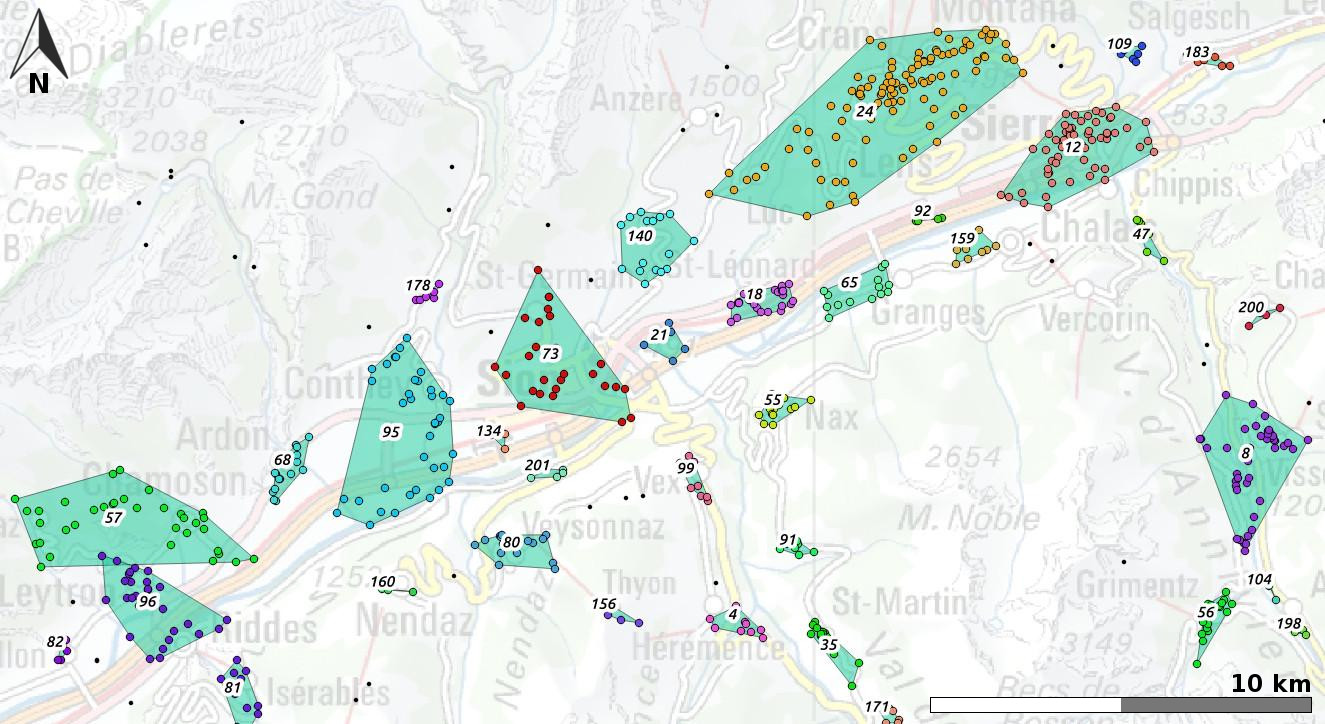
\includegraphics[width=0.8\linewidth]{clusters2.jpg}
\caption{A view of some resulting images clusters.}
\label{clusters}
\end{figure}


\subsubsection*{Matching}
%%%%%%%%%%%%%%%%%%%%%%%%%%%%%%%%%%%%%%%%
Then, by making the nearest neighbourg distance ratio of the SIFT matching 
procedure varying, we deduced its best value equals to 2/3 for our dataset.
Applying RANSAC improves the results (fig.\,\ref{res:2}), but our geometrical 
filter was much more better at this task (fig.\,\ref{res:3}).

\begin{figure}[H]
\centering
\begin{subfigure}{0.32\textwidth}
    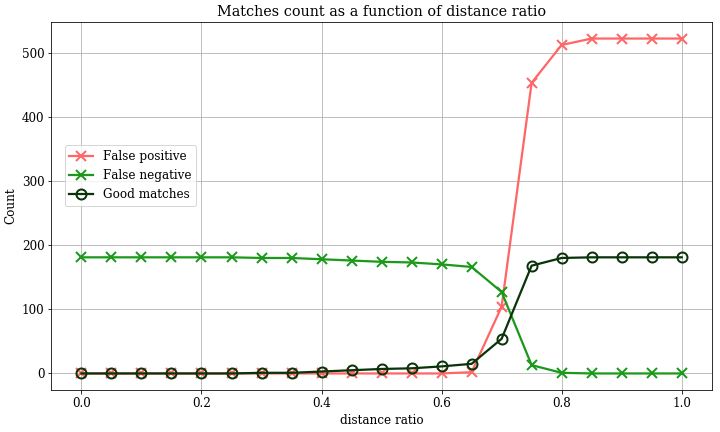
\includegraphics[width=1\linewidth]{res_1.png}
    \caption{After the simple matching.}
    \label{res:1}
\end{subfigure}
~
\begin{subfigure}{0.32\textwidth}
    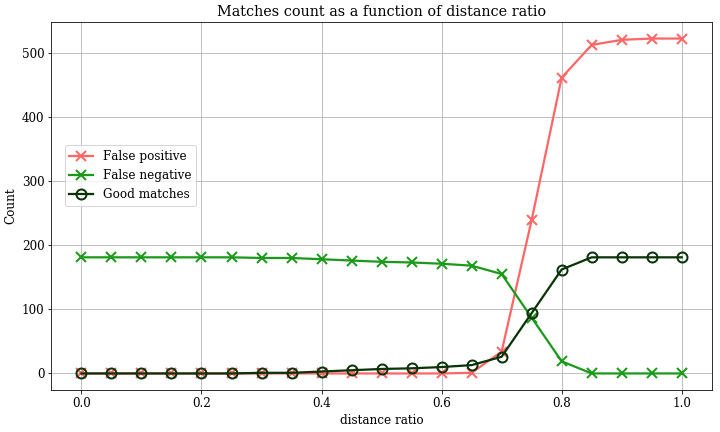
\includegraphics[width=1\linewidth]{res_2.png}
    \caption{After using RANSAC.}
    \label{res:2}
\end{subfigure}
~
\begin{subfigure}{0.32\textwidth}
    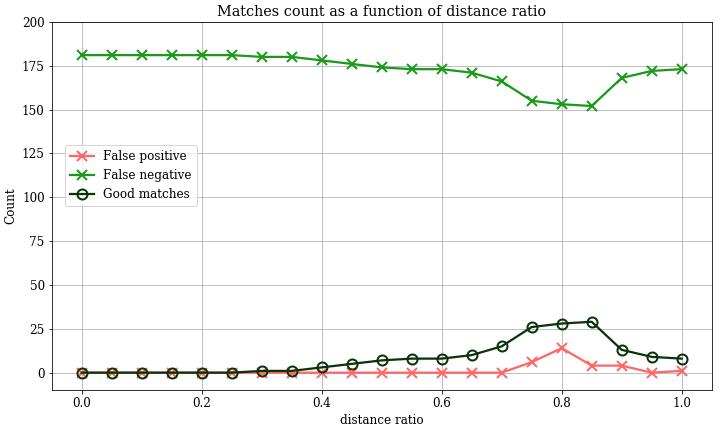
\includegraphics[width=1\linewidth]{res_3.png}
    \caption{After applying our filter.}
    \label{res:3}
\end{subfigure}
\caption[Results showing the improvement of the RANSAC and our filter]{Results showing the improvement of the RANSAC and our filter on the recall as a function of the nearest neighbor distance ratio used 
by the SIFT algorithm. \colorbox{yellow}{REDRAW LES FIGURES}}
\label{res}
\end{figure}

Others parameters of the SIFT and RANSAC algorithms were also tested (not showed here)
and led to the values in table \ref{values}.


\begin{table}[H]
\small
\centering
\begin{tabularx}{0.67\textwidth}{@{\extracolsep{\fill} } l l r  }
\makecell{Algorithm} & \makecell[l]{Parameter name} & \makecell[r]{Value used \\in this study} \\% & \makecell{Values used by \\ \citep{lowe1999} for SIFT}\\
\toprule[1pt]
\multirow{4}{*}{SIFT} & Number of octaves & 2 \\% &3  \\
 & Contrast threshold & 0.032 \\%&  0.04\\
 & Edge threshold & 18 \\%& 10 \\
 & Sigma & 1.2 \\%& 1.6 \\
\midrule[0.1pt]
\multirow{3}{*}{RANSAC} & Reprojection error [px] & 5 \\
 & Max. number of iterations & 2000 \\
 & Confidence level & 0.995 \\
\bottomrule[1pt]
\end{tabularx}
\caption{Retained values for the SIFT and RANSAC algorithms.}
\label{values}
\end{table}


\subsubsection*{Georeferencing}
%%%%%%%%%%%%%%%%%%%%%%%%%%%%%%%%%%%%%%%%
On the sample cluster, the 22 position results range from 15\,m to 8\,km (fig.\,\ref{pose:1}) and 3
were discarded because of a lack in DEM values (no data).



\begin{figure}[H]
\centering
\begin{subfigure}{0.48\linewidth}
    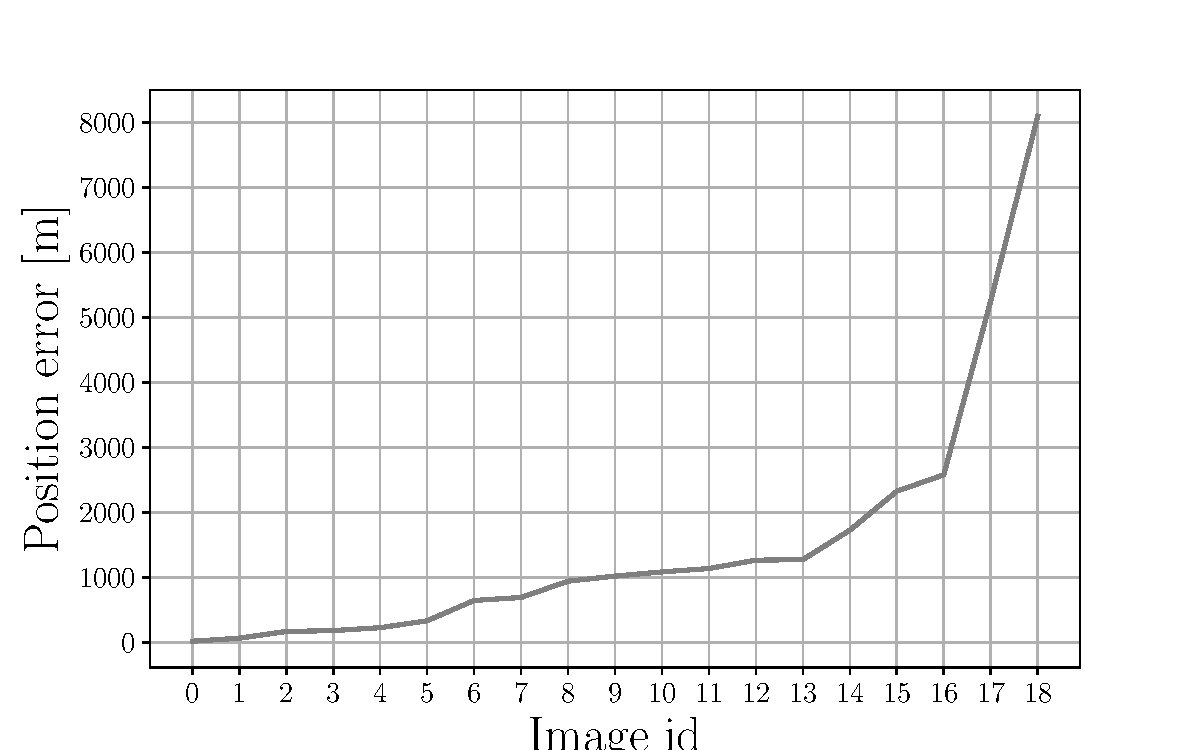
\includegraphics[width=1\linewidth]{pos.pdf}
    \caption{Position errors.}
    \label{pose:1}
\end{subfigure}
~
\begin{subfigure}{0.48\linewidth}
    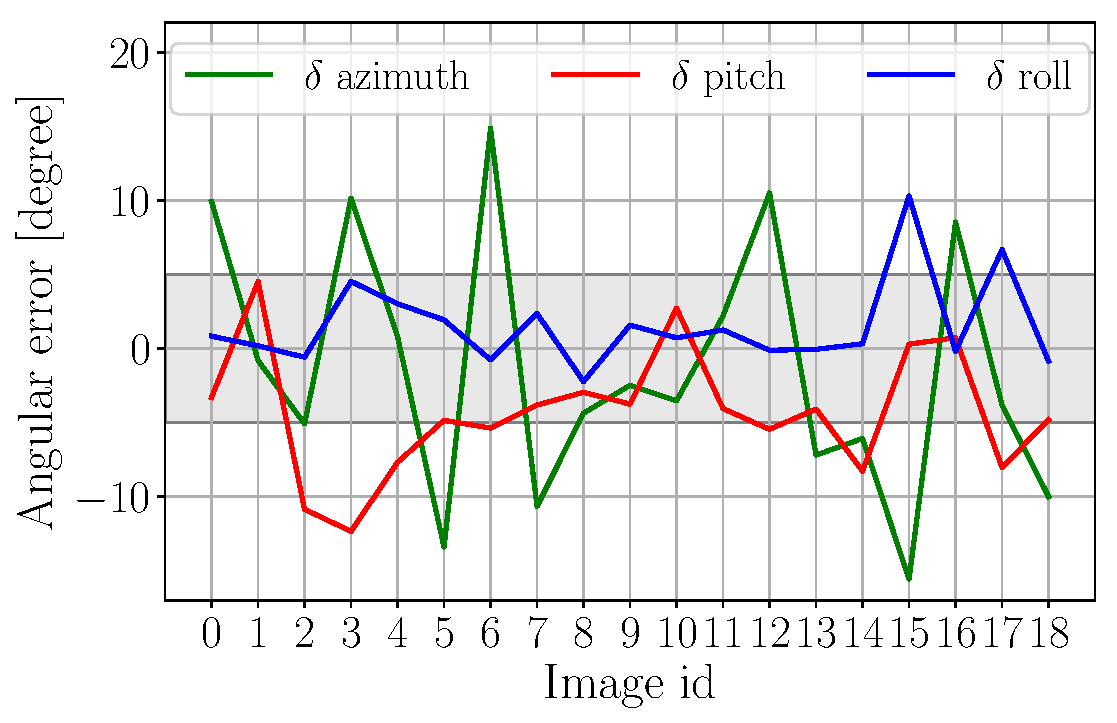
\includegraphics[width=1\linewidth]{angles.pdf}
    \caption{Angular errors. The [-5, 5] range is greyed out.}
    \label{pose:2}
\end{subfigure}
\caption{Camera pose (ground truth minus computed position) results on 19 query images.}
\label{pose}
\end{figure}




%%%%%%%%%%%%%%%%%%%%%%%%%%%%%%%%%%%%%%%%%%%%%%%%%%%%%%%%%%%%%%%%%%%%%%%%%%%%%%%%
\section*{Discussion}
%%%%%%%%%%%%%%%%%%%%%%%%%%%%%%%%%%%%%%%%%%%%%%%%%%%%%%%%%%%%%%%%%%%%%%%%%%%%%%%%
Results that are close to the user provided position (which is taken as ground truth) 
are often obtained when the camera was closed to the part of the landscape 
captured (fig.\,\ref{ex1}).

\begin{figure}[H]
\centering
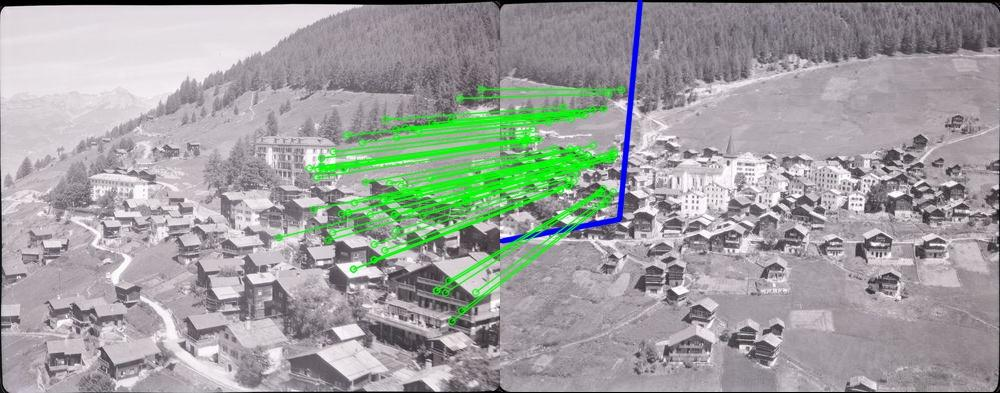
\includegraphics[width=0.8\linewidth]{ex1.jpg}
\caption[These two images show a pose result that is 15\,m to the position in database.]
{The pose result of the query image (right) is only 15\,m close to the position in database.\\
Images source: EPFL, Archives de la construction moderne.}
\label{ex1}
\end{figure}


In some cases, a large posiiton or angulair shifts may be explained by tie points 
not homogeneousely distributed on the images. In addition to a small overlap,
figure \ref{ex3} shows that tie points on these two images are almost along a 
vertical line. This may explained why the azimuth is ~16\textdegree away from the
database value.


\begin{figure}[H]
\centering
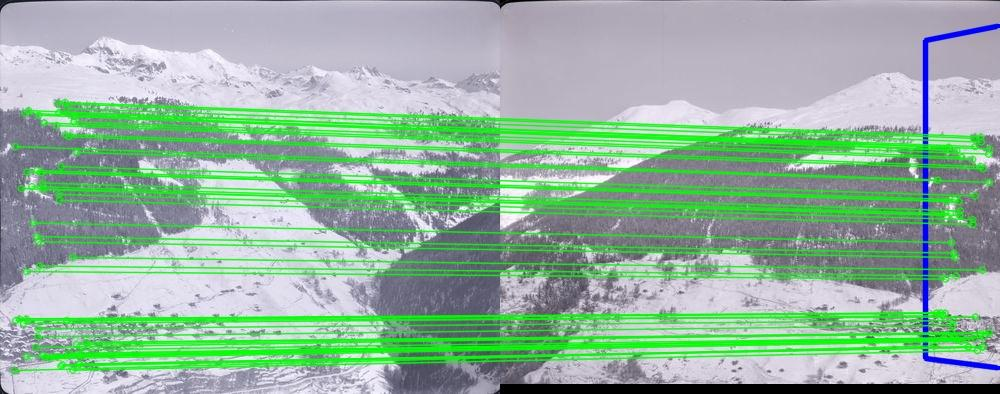
\includegraphics[width=0.8\linewidth]{ex3.jpg}
\caption[These two images show a pose result that is 2.3\,km and an azimuth that is 16\textdegree 
away from the position in database.]
{The pose result of the query image (right) is 2.3\,km and an azimuth 16\textdegree 
away from the values in database. \\
Images source: EPFL, Archives de la construction moderne.}
\label{ex3}
\end{figure}


Other position shifts are explained by tie points beeing located close to a breakline
in the image depth. Figure\,\ref{ex2:2} shows such a case; tie points are in the 
background on the images, but their 3D coordinates are taken on the forground on 
the DEM, which is approximately 2\,km away from their real location in the background.

\begin{figure}[H]
\centering
\begin{subfigure}{0.48\linewidth}
    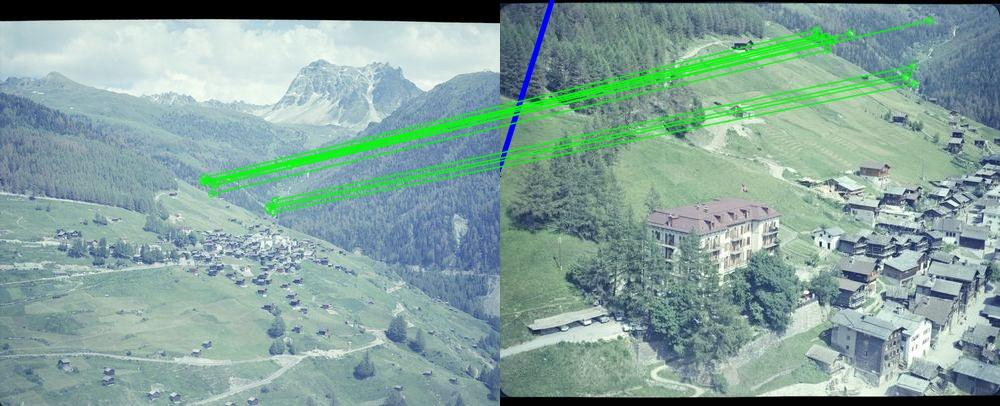
\includegraphics[width=1\linewidth]{ex2.jpg}
    \caption{Tie points are located near a breakline in the image depth.}
    \label{ex2:1}
\end{subfigure}
~
\begin{subfigure}{0.48\linewidth}
    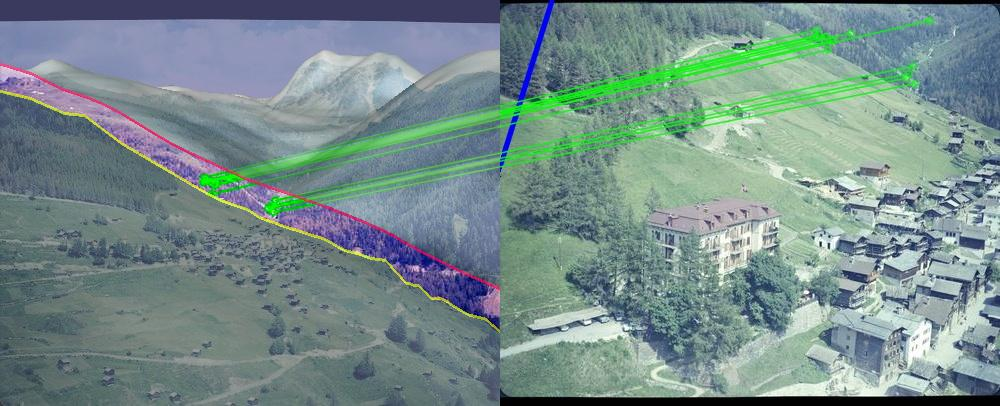
\includegraphics[width=1\linewidth]{ex2_mnt.jpg}
    \caption{When superimposed with the DEM, the breakline between the forground 
    and the background is higher on the DEM than on the image.}
    \label{ex2:2}
\end{subfigure}
\caption[]{The pose of the query image (right) is 1.7\,km away from its position in database.}
\label{ex2}
\end{figure}










%%%%%%%%%%%%%%%%%%%%%%%%%%%%%%%%%%%%%%%%%%%%%%%%%%%%%%%%%%%%%%%%%%%%%%%%%%%%%%%%
\section*{Conclusion}
%%%%%%%%%%%%%%%%%%%%%%%%%%%%%%%%%%%%%%%%%%%%%%%%%%%%%%%%%%%%%%%%%%%%%%%%%%%%%%%%
Results showed that the pose computation of a query image is quite accurate
when some conditons are respected;  the accuracy of the reference image
pose is crucial. It influences the DEM relative position and 3D coordinates of
tie points. The query image pose accuracy cannot be better than the reference one.

Tie points distribution on images is also of great importance as shown by this
study. An homogeneous distrubution would undoubtedly improve the precision of the
computed position.

This would also be the case if we can detect and use GCPs that are already 
in database to register a query image. 

%In this study, clustering was possible because images positions were already known.
Furthermore, as the Brute-Force matching process is a O(n$^{2}$) complex problem, 
it takes too much time to tackle any new large images dataset with no known 
a priori positions and where clusters cannot be built. This would need strong
computational power.
Reducing features space and avoiding to much redundancy would be ways to explore 
prior to the matching stage.
In such way, machine learning or bag-of-features techniques may offer other 
valuable alternative to find overlapping images.


Finally, to integrate this process on the web platform, we will need a two-steps
approach: 1) proposing overlapping images to the user and 2) once a picture has 
been successfully georeferenced by the user, giving him the possibility to see
which other images were automatically registred and giving him the opportunity
to refine the automatic results. Field of user engagement could for example 
help building a nice interface to improve and keep the users motivation in this 
great task.


%Finally, we still need to evaluate how to integrate this process on the web 
%platform, and how we can offer the user a friendly way to check and validate the 
%computation results. 



%%%%%%%%%%%%%%%%%%%%%%%%%%%%%%%%%%%%%%%%%%%%%%%%%%%%%%%%%%%%%%%%%%%%%%%%%%%%%%%%
%\section*{Acknowledgments}
%%%%%%%%%%%%%%%%%%%%%%%%%%%%%%%%%%%%%%%%%%%%%%%%%%%%%%%%%%%%%%%%%%%%%%%%%%%%%%%%


%%%%%%%%%%%%%%%%%%%%%%%%%%%%%%%%%%%%%%%%%%%%%%%%%%%%%%%%%%%%%%%%%%%%%%%%%%%%%%%%
\bibliography{biblio}
%%%%%%%%%%%%%%%%%%%%%%%%%%%%%%%%%%%%%%%%%%%%%%%%%%%%%%%%%%%%%%%%%%%%%%%%%%%%%%%%




















\iffalse

\newpage{}
%%%%%%%%%%%%%%%%%%%%%%%%%%%%%%%%%%%%%%%%%%%%%%%%%%%%%%%%%%%%%%%%%%%%%%%%%%%%%%%%
%%%%%%%%%%%%%%%%%%%%%%%%%%%%%%%%%%%%%%%%%%%%%%%%%%%%%%%%%%%%%%%%%%%%%%%%%%%%%%%%
\section*{Introduction}

Your introduction goes here! Some examples of commonly used commands and features are listed below, to help you get started.

If you have a question, please use the help menu in the top right of the screen to get in touch. When your article or pre-print is complete, use the "Submit to PeerJ" button in the topbar to send your files to PeerJ.

\subsection*{About PeerJ}

PeerJ is an award-winning open access publisher covering the biological and medical sciences.  PeerJ provides authors with three publication venues: \textit{PeerJ} and \textit{PeerJ Computer Science} (peer-reviewed academic journals) and \textit{PeerJ PrePrints} (a 'pre-print server'). See https://peerj.com/about/publications/ for more information.

The PeerJ model allows an author to publish articles in their peer-reviewed journal via the purchase of a lifetime Publication Plan. Prices start from just \$99 (a one-off payment) which entitles an author to the lifetime ability to publish 1 article per year for free. Publication in PeerJ PrePrints is entirely free.

\section*{Some \LaTeX{} Examples}
\label{sec:examples}

Use section and subsection commands to organize your document. \LaTeX{} handles all the formatting and numbering automatically. Use ref and label commands for cross-references.

\subsection*{Figures and Tables}

Use the table and tabular commands for basic tables --- see Table~\ref{tab:widgets}, for example. You can upload a figure (JPEG, PNG or PDF) using the project menu. To include it in your document, use the includegraphics command as in the code for Figure~\ref{fig:view} below.

\begin{figure}[ht]
\centering
\includegraphics[width=\linewidth]{view}
\caption{An example image.}
\label{fig:view}
\end{figure}

\begin{table}[ht]
\centering
\begin{tabular}{l|r}
Item & Quantity \\\hline
Widgets & 42 \\
Gadgets & 13
\end{tabular}
\caption{\label{tab:widgets}An example table.}
\end{table}

\subsection*{Citations}

LaTeX formats citations and references automatically using the bibliography records in your .bib file, which you can edit via the project menu. Use the cite command for an inline citation, like \cite{Figueredo:2009dg}, and the citep command for a citation in parentheses \citep{Figueredo:2009dg}.

\subsection*{Mathematics}

\LaTeX{} is great at typesetting mathematics. Let $X_1, X_2, \ldots, X_n$ be a sequence of independent and identically distributed random variables with $\text{E}[X_i] = \mu$ and $\text{Var}[X_i] = \sigma^2 < \infty$, and let
$$S_n = \frac{X_1 + X_2 + \cdots + X_n}{n}
      = \frac{1}{n}\sum_{i}^{n} X_i$$
denote their mean. Then as $n$ approaches infinity, the random variables $\sqrt{n}(S_n - \mu)$ converge in distribution to a normal $\mathcal{N}(0, \sigma^2)$.

\subsection*{Lists}

You can make lists with automatic numbering \dots

\begin{enumerate}[noitemsep] 
\item Like this,
\item and like this.
\end{enumerate}
\dots or bullet points \dots
\begin{itemize}[noitemsep] 
\item Like this,
\item and like this.
\end{itemize}
\dots or with words and descriptions \dots
\begin{description}
\item[Word] Definition
\item[Concept] Explanation
\item[Idea] Text
\end{description}

We hope you find write\LaTeX\ useful for your PeerJ submission, and please let us know if you have any feedback. Further examples with dummy text are included in the following pages.

\section*{Methods}

\lipsum[4] % Dummy text

\begin{equation}
\cos^3 \theta =\frac{1}{4}\cos\theta+\frac{3}{4}\cos 3\theta
\label{eq:refname2}
\end{equation}

\lipsum[5] % Dummy text

\subsection*{Subsection}

\lipsum[6] % Dummy text

\paragraph{Paragraph} \lipsum[7] % Dummy text
\paragraph{Paragraph} \lipsum[8] % Dummy text

\subsection*{Subsection}

\lipsum[9] % Dummy text

\begin{figure}[ht]\centering
\includegraphics[width=\linewidth]{results}
\caption{In-text Picture}
\label{fig:results}
\end{figure}

Reference to Figure \ref{fig:results}.

\section*{Results and Discussion}

\lipsum[10] % Dummy text

\subsection*{Subsection}

\lipsum[11] % Dummy text

\subsubsection*{Subsubsection}

\lipsum[12] % Dummy text

\subsubsection*{Subsubsection}

\lipsum[14] % Dummy text

\subsection*{Subsection}

\lipsum[15-20] % Dummy text

\section*{Acknowledgments}

So long and thanks for all the fish.

\bibliography{sample}
\fi




\end{document}